\subsection{Architectural Views}

\subsubsection{Logical View} % which is the object model of the design, end-user functionality (Class diagrams)

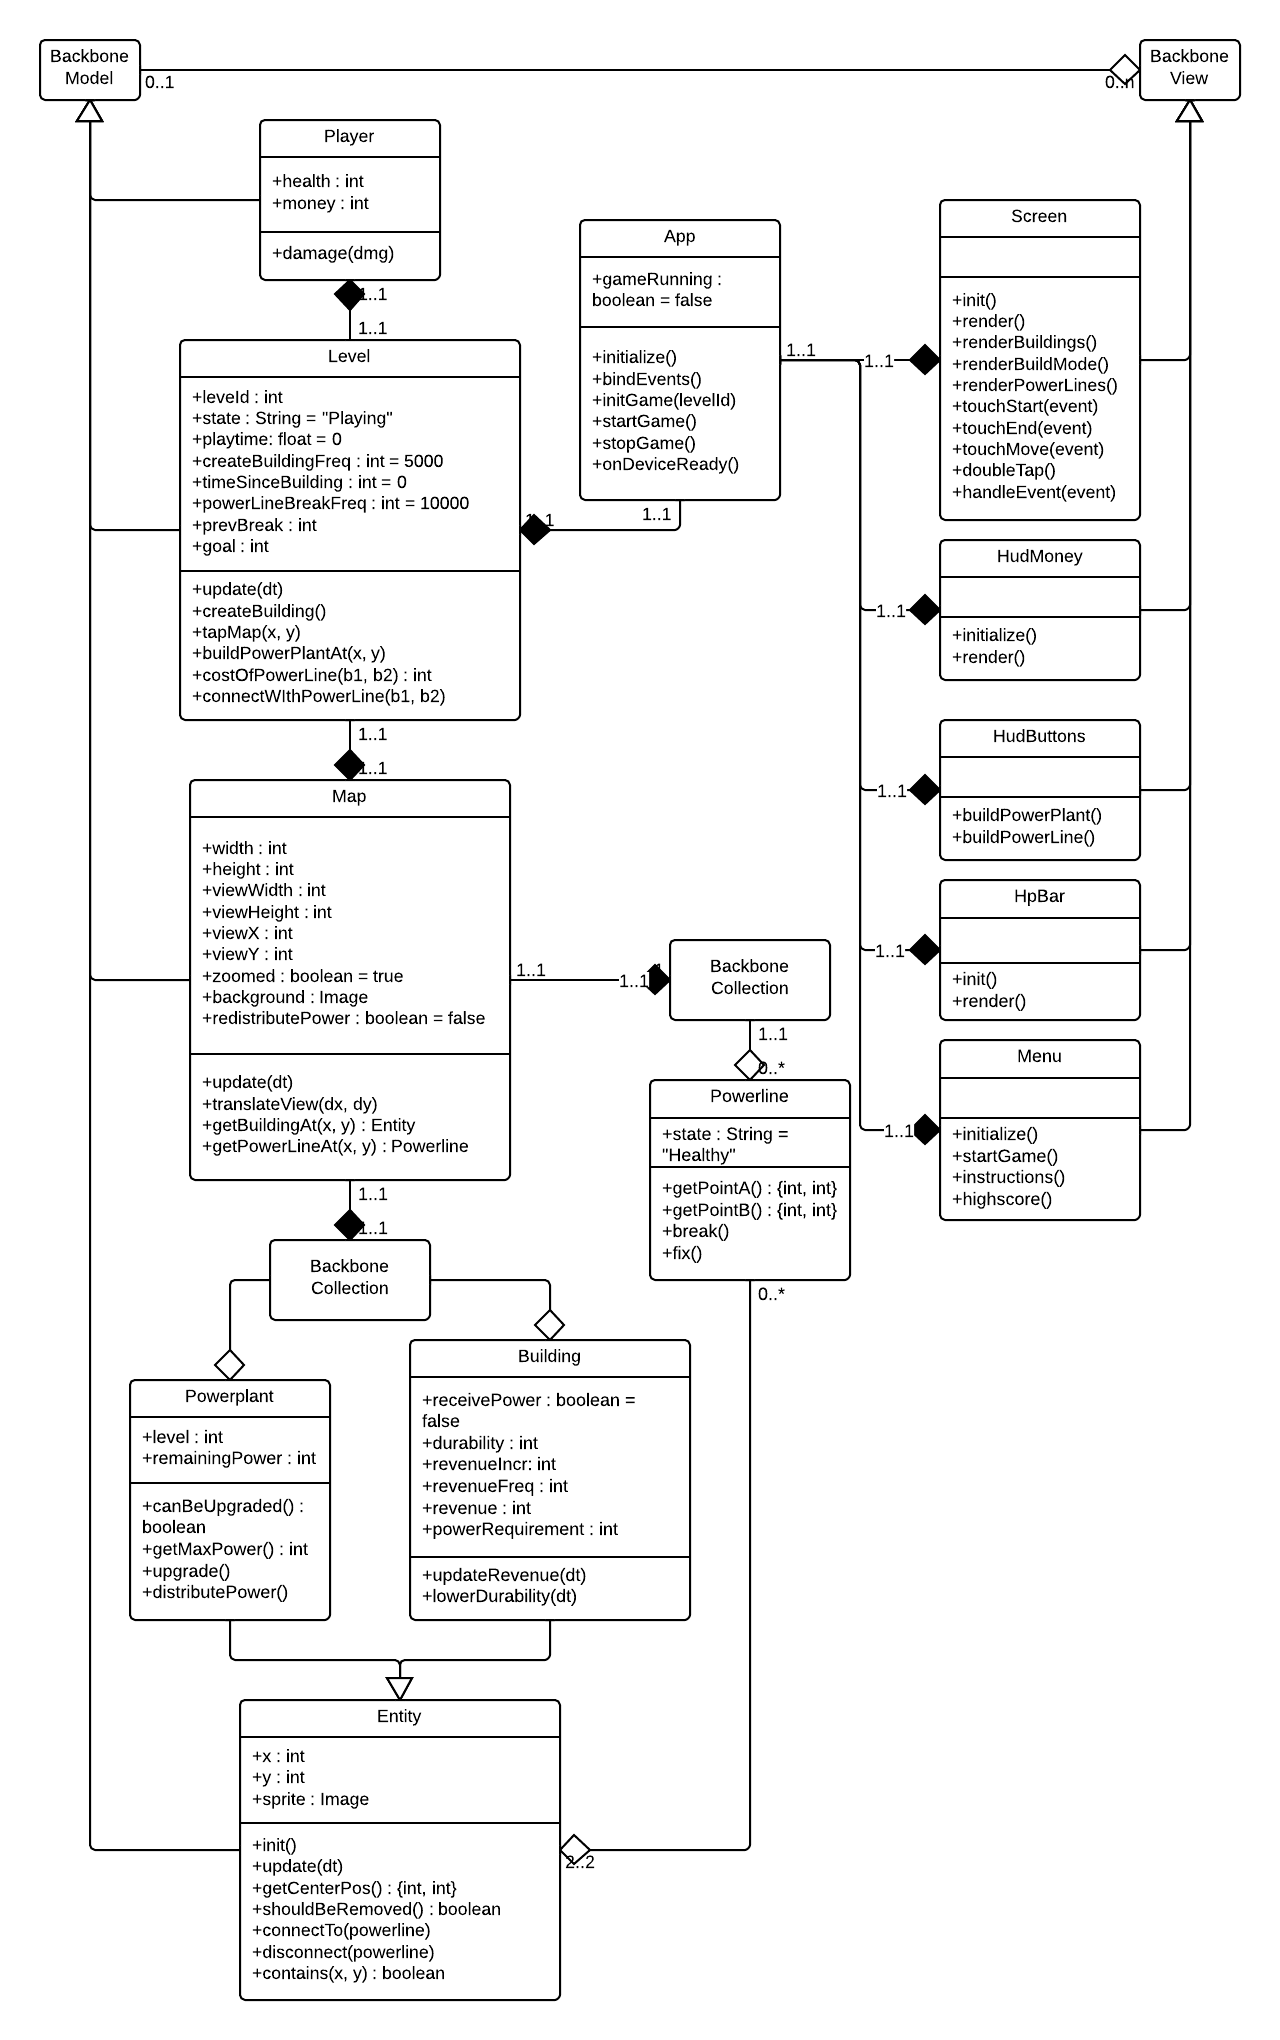
\includegraphics[width=\textwidth]{pictures/class_diagram}

-->> The screen class will probably become connected to more classes as the GUI is planned. <<--

\subsubsection{Process View} % captures the concurrency and synchronization aspects of the design, itegrators, performance, scalability. Takes into account some non-functional requirements, like performance and reliability.
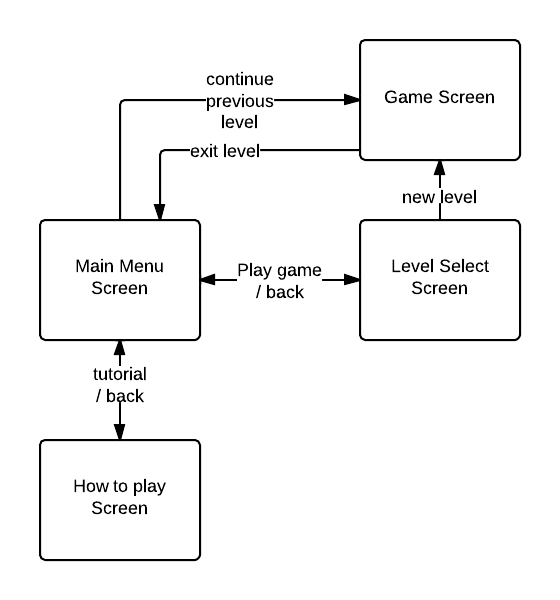
\includegraphics[width=\textwidth]{pictures/process_view_screen_flow}

The main menu screen is the entry point for the game. From there you can go to the how to play screen, 
to read about how the game works. You can go to the Level Select screen to start a new level, or load the 
most recent level and continue playing from where you last left of. While playing you can exit the current 
level and return to the main menu.

\subsubsection{Physical View} % describes the mappings of the software onto the hardware, and reflects its distributed aspect, system engineers, topology, communications

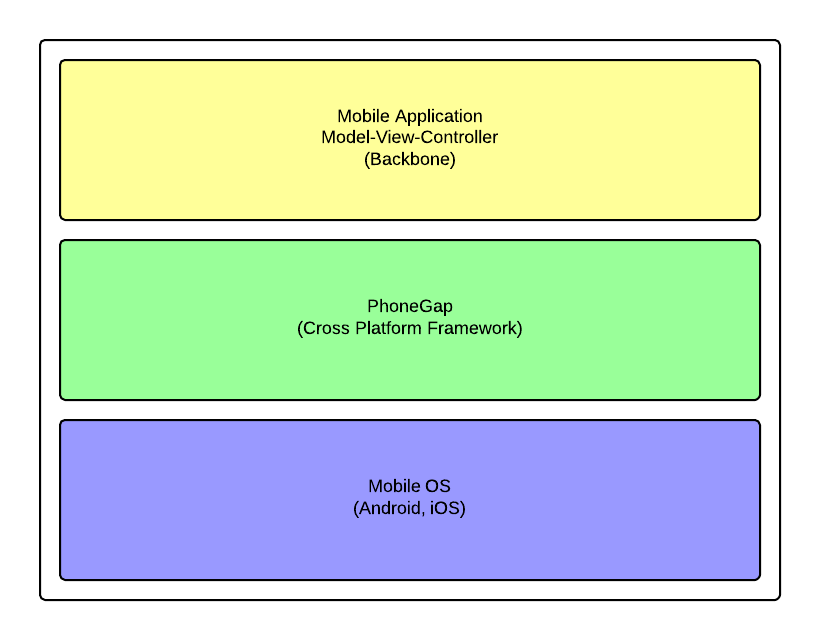
\includegraphics[width=\textwidth]{pictures/physical_view}

The physical architecture of our product is seperated into 3 layers. Platform specific issues are handled 
using PhoneGap as a cross platform framework between the application and the mobile OS.

{\bf Layer 1 - Native platform}
The first layer is the native operative system that runs on the device. This layer handles touchscreen 
functionality, rendering to screen, data input/output and other platform specific features.

{\bf Layer 2 - Cross platform framework}
The cross platform framework is called PhoneGap. The purpose of this layer is to allow the development 
team to write portable code that can run on both Android and iOS, without having to develop for both 
Android and iOS separately in 2 different programming languages. PhoneGap uses browser functionality on 
each platform to run HTML5, CSS and JavaScript code and provides access to platform functionality like 
camera and touchscreen.

{\bf Layer 3 - Mobile Application}
The third layer is where the game is implemented using the MVC pattern with Backbone. 


\subsubsection{Development View} % describes the static organization of the software in its development environment, programmers, software management
The development view is separated into hierarchically into layers. The Game Assets layer contains 
singleton objects with assets like images and preallocated objects. The game logic layer is where 
the game itself runs. The PhoneGap layer is a cross platform layer which allows our code to run on 
different devices. The final layer is the Platform specific SDK.

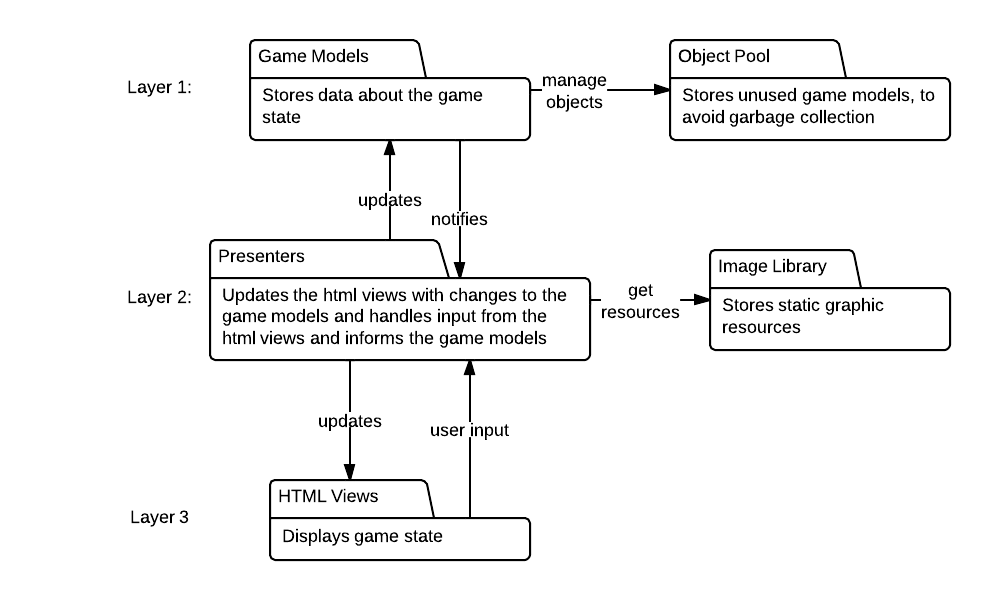
\includegraphics[width=\textwidth]{pictures/development_view}
